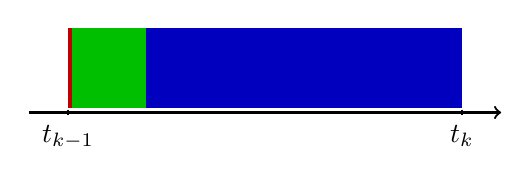
\begin{tikzpicture}
\definecolor{green}{RGB}{0,190,0};
\definecolor{red}{RGB}{190,0,0};
\definecolor{blue}{RGB}{0,0,190};
%Draw bounding box
%\draw (-2.75,-1.75) rectangle (3.75,3.25);

%Draw time line
\draw[ thick, ->] (-.5,-2pt) -- (5.5,-2pt);

\draw[thick]  (5 cm, -1pt)  -- (5 cm, -3pt) node[anchor=north] {$t_{k }$ };
\draw[thick]  (0cm , -1pt)  -- (0 cm, -3pt) node[anchor=north] {$t_{k-1}$ };

%Solve for control in t_k-1
\draw[red,fill=red] (0,0) rectangle (0.05, 1);
% Calculcate start value for t_k
\draw[green, fill=green] (0.05,0) rectangle (1, 1);
%Prepare for t_k
\draw[blue,fill=blue] (1,0) rectangle (5,1);

\end{tikzpicture}